In this chapter, we discuss the overall project design of our system, the tasks, and the used tools for each task.
\label{chapter_project_design}
%-----------------------------------------------------%
%-----------------------------------------------------%
%-----------------------------------------------------%

\section{Technical Specifications}
\label{tech_specs}
In this section, we explain the project's technical specifications regarding autonomous functionalities, communication, and cooperation. Autonomous functionalities deals with the design of an autonomous car that is capable of decision making. Communication deals with how information about every AV is transferred to its neighbouring ones regarding the message structure. Cooperation deals with the solutions to make the AVs clear the traffic for the EV through reinforcement learning.  

%-----------------------------------------------------%

\subsection{Environment and Agent Model}
\label{specs_env_agent_mdl}
In this subsection, we introduce our simulation environments: Gazebo \cite{Koenig04designand} and SUMO \cite{sumomain}, each of which was chosen for a different specific purpose. In order to simulate the realistic dynamics of our vehicles and implement the different autonomous functionalities they should be capable of performing, we chose to use Gazebo on the Robotics Operating System (ROS)\cite{ROSBookMorgan}. On the other hand, for the sake of training and testing our reinforcement learning model and measuring aggregate system metrics, we chose SUMO. All the same, upon fully training the model, we then deploy it on our fully functional autonomous vehicles in Gazebo.\\
For each of the two simulation environments, we provide a brief description as well as present the used tracks (assumptions/ specifications/dimensions). We also demonstrate our agent model (sensors and mechanics) in both Gazebo and SUMO.

\subsubsection{Gazebo}
\begin{itemize}
    \item \textbf{Gazebo Environment}
    \\ \\ Gazebo is an open-source 3D multi-robot simulation environment\cite{Koenig04designand}. By far the most attractive characteristic of Gazebo is that it is compatible with the Robotics Operating System (ROS) which we are using. ROS is an open-source, meta-operating system used for multitudes of robotics applications\cite{ROSBookMorgan}. Owing to the several useful services it provides, such as hardware abstraction and inter-processes message-passing\cite{ROSBookMorgan}, ROS is used as our basic framework in developing our system of autonomous vehicles. 
    \\ \\From another perspective, what makes Gazebo quite an enticing choice of a simulation environment is its remarkable degree of realism\cite{Koenig04designand}; it greatly cuts down on the effort of transferring simulated systems into functional ones on real hardware. This can be inferred from its following features:

    \begin{enumerate}
        \item Gazebo allows the rendering of realistic 3D environments, allowing for the simulations of textures and lighting\cite{Koenig04designand}. In order not to complicate our simulated scenarios, we used Gazebo to design our track to be a simple straight three-lane road as demonstrated in Figure \ref{fig:3Lanes_fig}. The lanes are numbered 0-2, where lane 0 is the left-most one. Since our adopted agent model is that of a vehicle scaled down ten times, as discussed in \ref{specs_gaz_agent}, our road width is set to 1.575 meters (each of the three lanes is 0.525 meters wide) and our road length is set to 100 meters. 
        \\ \\ In order to better define and simplify our simulated track, the road was designed with the following underlying assumptions:
        \begin{itemize}
            \item The ground is smooth; no bumps or pits exist.
            \item The track is perfectly straight without any intersections or merges.
            \item The road is black and the lane lines are white to facilitate lane detection.
            \item The road is sufficiently lighted.
            \item There are no pedestrians involved.
            \item Other vehicles are the only dynamic obstacles on the road.
        \end{itemize}
        
        \begin{figure}[h]

        \centering
        \begin{subfigure}{0.5\textwidth}
        \hspace*{2cm}
        
\includegraphics[width=0.75\linewidth, height=5cm]{3Lanes1} 
        %\quad
        \label{fig:3Lanes1_fig}
        \end{subfigure}
        \begin{subfigure}{0.5\textwidth}
        \hspace*{2cm}
        
\includegraphics[width=0.75\linewidth, height=5cm]{3Lanes2}
        %\quad
        \label{fig:3Lanes2_fig}
        \end{subfigure}
        
        \caption{Straight three-lane road simulated in Gazebo.}
        \label{fig:3Lanes_fig}
        \end{figure}
        
        \item Gazebo provides a simple API for adding any new model to the environment. Models include anything from arbitrary stationary objects to whole dynamic robot models\cite{Koenig04designand}. In our case, an example of added stationary models are the sidewalks and construction barrels, while autonomous vehicles are our only simulated dynamic objects. 
        
        \item Gazebo is built on top of The Open Dynamics Engine, a high-performance physics engine which allows for simulation of the realistic dynamics and kinematics of rigid bodies\cite{Haber2012jmeSimAO}. This allows us to simulate our autonomous vehicles and their control with a relatively acceptable degree of accuracy.
        
        \item A very important aspect of Gazebo is that it not only allows for simulating numerous actuators and sensors\cite{Koenig04designand}, but it is also capable of obtaining noisy measurements from these sensors so that their performance better matches that of the real hardware sensors.
        
        \item Gazebo supports more than one choice of update rates of the simulation environment. The update rate could either be manually specified by the user, or the simulator could be prompted to attempt running in real time or as fast as possible. In our simulations, we use Gazebo’s default setting; which is attempting to run in real time or as fast as the machine can handle.
    \end{enumerate}

    \item \textbf{Gazebo Agent Model}
    \label{specs_gaz_agent}
    \\ \\Our Agent model is adapted from the F1/10 platform which introduces a fully autonomous Ackerman steering race robot inspired by the formula one race car. It is named F1/10 as it is 1/10 scale of an actual formula race car. This platform helps in making vehicle autonomy in a way that makes it easy to develop and implement different algorithms like perception, planning and control. F1/10 platform was first created in 2015 and is being continuously updated by its developers to break into autonomous racing. It is an open source project and is well documented on the official website f1tenth.org \cite{okelly2019f110}\cite{varundev_ros_19}. \\ 
    \\
Our agent in Figure \ref{fig:agent_model} is mimicking an actual  1/10 RC race car, traxxas xo-1, which is similar to the Tesla car  Model S. Thus, we make sure that our model will have similar dynamics to that of a full scale car. Moreover, the sensors used in the model are similar to those used in full scale autonomous cars except for their limited specifications. The Agent model has the following sensors; Hokuyo Laser Scanner, Black and White camera, and Vesc: an open source electronic speed controller \cite{okelly2019f110}.
    \begin{figure}[htbp]
    \centering
    \begin{subfigure}[t]{0.3\textwidth}
        \centering
        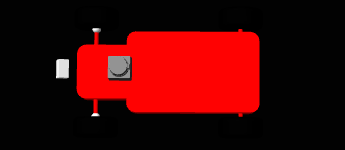
\includegraphics[width=1\linewidth, height=2.5cm]{images/racecar_topview.png}
        \caption{Agent model-Top view.}
        \label{fig:racecar_topview}
    \end{subfigure}\hfill
    \begin{subfigure}[t]{0.3\textwidth}
        \centering
        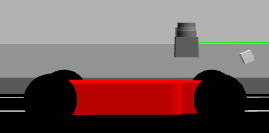
\includegraphics[width=1\linewidth, height=2.5cm]{images/racecar_sideview.png}
        \caption{Agent model-Side view.}
        \label{fig:racecar_sideview}
    \end{subfigure}\hfill
    \begin{subfigure}[t]{0.3\textwidth}
        \centering
        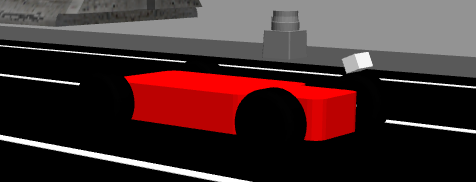
\includegraphics[width=1\linewidth, height=2.5cm]{images/racecar_isometricView.png}
        \caption{Agent model-Isometric view.}
        \label{fig:racecar_isonmetricview}
    \end{subfigure}\hfill
    \caption{Agent model spawned in Gazebo environment}
    \label{fig:agent_model}
    \end{figure}
    The sensors used in this model are for different purposes and are fused together to have a fully functional car:
    \begin{enumerate}
        \item \textbf{The Laser scanner} \\
    The Laser scanner is used for obstacle detection and can be utilized in mapping, localization and navigation \cite{HokutoLidar}. The one in our model is 270$^{\circ}$ wide detection angle with minimum range 0.1m and maximum range 10m at a 0.01 resolution, see Figure \ref{fig:270_deg_scan}. It is the grey object at the top of the AV in Figure \ref{fig:agent_model}.\\
    \begin{figure}[!h]
    \centering
    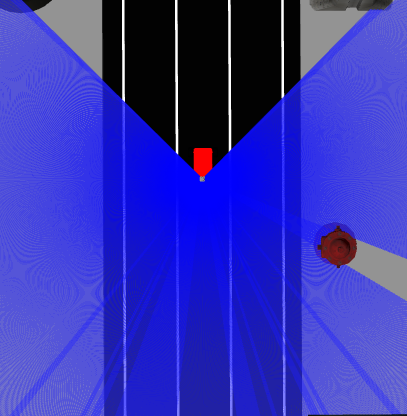
\includegraphics[height= 5cm,width=5cm]{images/270deg_scan.png}
    \caption{270$^{\circ}$ wide detection angle of the laser scaner.}
    \label{fig:270_deg_scan}
    \end{figure}
    \item \textbf{The Black and White camera} 
    \\ \\The camera is a black and white camera with image size 1280x1024 pixel. At the front of the vehicle, 0.08m above its center, with negative angle of 0.4 radians for it to have a good view of the lane lines. Also, its horizontal field of view is about 1.4 radians.\\
    \item \textbf{VESC}
    \\ \\The vesc is used to drive the brushless dc motor and control the speed, current, voltage, PWM and different parameters \cite{VESC_6_MKIV}. It also controls the servo motor and the steering accordingly, and publishes the vehicle velocity and yaw.\\
    \end{enumerate}
    
    Our Agent motion model is an Ackerman drive model \cite{okelly2019f110}. In order to avoid problems with wheels slipping and the inaccuracies with the robot motion; ackerman model was introduced in \cite{Kaltenegger2016a}\cite{10.5555/983690}, see Figure \ref{fig_ackerman_steering}. This is done by maintaining a reference centre point about which all the tires are rotating, and the angle of each tire with respect to this reference point varies from one tire to another; $\phi_{R}$ $>$ $\phi_{L}$ in Figure \ref{fig_ackerman_steering}. Also, each tire path has a different radius curvature to the reference point; each tire has different rotational speed accordingly. Under this design, the vehicle can rotate smoothly on high speeds without facing slipping problems, also avoiding any rolling over\cite{Kaltenegger2016a}.\\
    \begin{figure}[htbp]
    \centering
    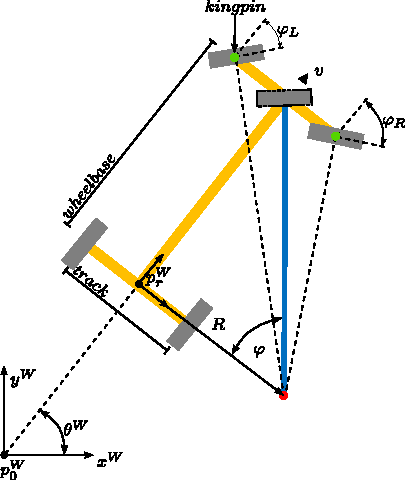
\includegraphics[height= 7cm,width=7cm]{images/AckermanSteering.pdf}
    \caption{The geometry of the ackermann robot in the two dimensional space \cite{Kaltenegger2016a}.}
    \label{fig_ackerman_steering}
    \end{figure}

\end{itemize}

\subsubsection{SUMO}
\begin{itemize}
    \item \textbf{SUMO Environment}
\\ \\SUMO simulation is an open source microscopic and continuous simulation package. It is mainly built for traffic management and vehicular communications. SUMO\cite{sumo_2012} provides the functionality of building roads, controlling their traffic signals and controlling Vehicles along with facilitating communication between them. SUMO developers, mainly from the  Institute of Transportation Systems at the German Aerospace Center, built a python API that is regularly updated through active discussions with the community. SUMO suite consists of four main applications:
\begin{enumerate}
    \item \textbf{Road Network Generation} 
    \\ \\SUMO road networks mimic real world roads by representing them as graphs where intersections are treated as nodes and roads are treated as edges. We used the SUMO application “netgenerate” to design a simple road network of three nodes and two edges, similar to that highlighted in Figure \ref{fig:3Lanes_fig} in the case of Gazebo. The first two nodes are used for vehicle placing with the first used for initializing the EV while the second is used for initializing agents. A distance ranging from 40 to 250 meters separating the two nodes was enforced to allow for variant interaction scenarios between the agents and the EV. Finally, the third node was set to be the end of the track where vehicles exit the simulation.\\
    
    \item \textbf{Vehicles and Routes}
    \\ \\Being a micro-simulation package, SUMO provides the functionality for deploying individual vehicles with a given set of parameters such as departure time, vehicles geometry, maximum allowed speed and vehicle types. For our purposes, we define two vehicle types:
    \begin{itemize}
        \item \textbf {Emergency vehicle}: To which the EV belongs. 
        \item \textbf {Ego vehicle}: A type defined for  agents in the simulation.
    \end{itemize}
	In addition to the parameters mentioned, each type is assigned a route to follow consisting of the start node, the destination node, and the edges connecting them.\\
	
    \item \textbf{Simulation} 
    \\ \\The application “sumo” launches a simulation of a previously configured network, our 3-lane network in this case. The simulation time is discretized, with a default simulation step size of 1 second. During simulation, vehicles navigate through the network according to the route specified by their type.
    \\We used the application “sumo” to perform a series of simulation epochs in our RL algorithm to allow agents a near realistic experience with the environment. Hence, rewards and Q table updates are iteratively performed after every epoch.\\
    
    \item \textbf{On-Line Interaction} 
    \\ \\SUMO  provides the ability to interact with an external application via a socket connection. This is done through the python interface TraCI: “Traffic Control Interface”, which facilitates controlling and retrieving vehicles states such as: speed, lane, position, as well as communicating this information between the vehicles. We also made use of TraCI in checking action feasibility. For instance: checking whether an agent is able to change lane (left/right) or accelerate.\\
    
\end{enumerate}

\item \textbf{SUMO Agent Model}
\label{sumo_agent_model}
\\ \\As discussed, SUMO is a microscopic simulator used to measure macroscopic properties of a traffic system; therefore, it provides control over vehicle actions, but in an accessible interface and -more importantly- simplified mechanical models. In the paragraphs below, we discuss the simplified vehicle-modelling approach allowing SUMO to achieve its goal in a computationally efficient manner.
\begin{enumerate}
    \item First and foremost, SUMO is \textbf{a top-view 2-dimensional simulator}, so it completely ignores any vertical (z-axis) forces. The concept of road-bumps or suspension mechanisms, for example, is non-existent. This is justified by the fact that these forces are irrelevant to the goal of traffic simulation, they are only useful for mechanics simulation, which is addressed in our ROS implementation.
    
    \item Since SUMO allows microscopic actions (eg: Lane change, Lane keeping, acceleration, and deceleration), it must adopt an agent-mechanics model; the vehicle bicycle model is chosen for this purpose.
    
    \item SUMO is a discrete-time continuous-space simulation environment, meaning that it updates the vehicles’ positions in time-steps $\Delta t$ moving them by a positional increment $\Delta x(t) =  \Delta t \; . \; (v(t) + \Delta t \; . \; a(t))$, where $a(t)$ is the acceleration chosen by the underlying car-following mode (see Point \ref{carfollower_pt}). This equation (called first order Euler scheme) simplifies the mechanics by assuming that the vehicle travels at a fixed speed within a time step and changes this speed instantaneously in between two steps. The instantaneity of actions is discussed more in Point \ref{instantaneity_pt}.\\ 
    The ``discrete-time" property also means that any possible actions to be taken by the agent should take the same amount of time = 1 time step = $\Delta t$, which is a simplifying assumption allowing granular yet simulator-orchestrated user-control for each vehicle; where the user gains control over each vehicle after each time step, further facilitating its use for RL applications.

    
    \item For longitudinal control, SUMO implements a set of car-following models\cite{sumomain}, assigning Krauss model\cite{kraussnewmod} by default, which is the one used in our autonomous agents; it is not used in the case of RL agents though- more on that in Point \ref{RL_pt}. The model, further discussed in \ref{specs_long_ctrl}, produces a safe desired “follow velocity” for the following (i.e. behind) vehicle to undertake, allowing it to maintain minimum-gap from the leading vehicle at all times. In the absence of a leading vehicle, the following vehicle uses its maximum allowable velocity.\\
    For lateral control, SUMO's default lane-changing model\cite{sumo_krauss} is used, with turning-off all automatic (strategic/ cooperative/ tactical/ regulatory) lane changes, specifically using \href{https://sumo.dlr.de/docs/TraCI/Change_Vehicle_State.html#lane_change_mode_0xb6}{lane change mode \textbf{512}} from SUMO's options. 
    \label{carfollower_pt}
    
    \item One simplifying and helpful feature of SUMO is instantaneity: At the moment the user retrieves control over each vehicle from SUMO (between each two time steps), the user can utilize SUMO's functionalities to set the speed of the vehicle for the next step instantaneously, as opposed to increasing the velocity gradually over the next time step. This reveals one simplification of SUMO: it does not simulate based on force/mass but rather on velocity/acceleration, ignoring some dynamical aspects such as inertia and force-reactions.\\
    The instantaneous speed, however, is limited by the agent's maximum possible velocity, acceleration, and deceleration.
    \label{instantaneity_pt}
    
    \item For each individual vehicle, SUMO provides a set of controllable parameters, the ones we used were:
    \begin{itemize}
        \item vehicle's maximum speed: set to 10 cells/sec in the EV, and 5 cells/sec in the agent vehicle.
        
        \item  vehicle's maximum acceleration: set to 2 cells/sec$^2$ for the EV, and 1 cells/sec$^2$ for the agent vehicle.
        
        \item vehicle's minimum acceleration (maximum deceleration): set to -2 cells/sec$^2$ for the emergency vehicle, and -1 cells/sec$^2$ for the agent vehicle. It is important to note here that: vehicles in SUMO can not move backwards, so that the minimum possible velocity of any vehicle is zero.
        
        \item minimum gap for following vehicle to keep: 2.5 cells for both emergency and agent vehicle.
        
        \item vehicle length: set to 2 cells for both EV and agent vehicle.
    \end{itemize}
    The larger speed for the EV compared to our agent is assigned in similarity to typical real environments, where emergency vehicles are allowed larger speeds. These parameters are maintained in all our experiments.
    
    
    \item On associating each of our agents with a control model, in our experiments we use the models defined below:
    \begin{itemize}
        \item \textbf{SUMO\_KRAUSS }: name for the SUMO-controlled autonomous vehicles. These vehicles have automatic lane changes turned off, and try to reach their maximum safe speed using Krauss model mentioned in Point \ref{carfollower_pt}. These vehicles are also \textbf{not} aware of the presence of the EV. They also avoid making any accidents.
        
        \item \textbf{Q\_LEARNING\_SINGLE\_AGENT} : Our RL-controlled vehicles. These vehicles have automatic lane changes turned off, and leave the option for the RL algorithm (Q\_learning, in our case) to choose between the list of its possible actions given the observed state; more on this later. These vehicles are aware of the presence of the EV. They also avoid making any accidents.
        
    \end{itemize}
    \label{RL_pt}
    
\end{enumerate}
\end{itemize}
%-----------------------------------------------------%

\subsection{Autonomous Functionalities}
\label{specs_auto_func}
In this subsection we explain how the autonomous functionalities are designed. The explained functionalities are: mapping, localization, longitudinal control, lateral control, lane keeping, lane changing, path planning, navigation, external commands following, and the high-level control master. 

\subsubsection{Mapping and Localization}
\label{specs_loc_map}
The AV has to be capable of mapping its environment as well as localize itself in it. The following points discuss the main approaches used for those purposes, which we also adopt in our implementation.
\begin{enumerate}
\item \textbf{Mapping} 
\\ \\
Gmapping is probably most used in SLAM algorithm, its problem formulation has the observations and odemoetry measurements as the givens and the posterior and a grid map as the result. The main key idea of Gmapping is that it depends on an advanced particle filter algorithm called Rao-Blackwellized particle filter \cite{4084563}\cite{OpenSlam}. Each particle is considered to be a sample of history of robot poses and posterior over maps given the sample pose history; approximate posterior over maps by distribution with all probability mass on the most likely map whenever posterior is needed. Each particle in the particle filter carries an individual map of the environment and hence contributes to generating a collective output map \cite{thrun2005probabilistic}. 

\item \textbf{Localization} 
\\ \\
In order for the robot to navigate in a  provided map, it must first be able to localize itself in it. This can be done using the AMCL algorithm. The AMCL algorithm, or the adaptive Monte Carlo localization algorithm, is a probabilistic localization algorithm which uses a particle filter to determine the robot position and orientation in a given map \cite{10.5555/2566804}. 
The AMCL algorithm takes as input the map, the robot’s laser scans, the mean and covariance of the robot's initial position and the transform messages. The algorithm outputs the mean and covariance of the robot’s estimated position, the estimated positions of the particles in the filter, and the transformation \cite{10.5555/2566804}\cite{ROSRoboticsProjects}. Note that the AMCL algorithm has a lot of parameters, like the minimum and maximum number of particles that we set to be their default values.

\end{enumerate}

%-----------------------------------------------------%
\subsubsection{Longitudinal Control}
\label{specs_long_ctrl}
One primary functionality that our autonomous vehicle should be capable of performing is regulating its driving speed as necessary. It has to be able to determine the appropriate velocity that it needs to move with at all times and then carry out the suitable throttle/brake commands accordingly \cite{LongCtrl}. This is achieved by the vehicle’s longitudinal controller. \\ \\
For the velocity generation task, we chose to implement the car-following model named Krauss model \cite{Krau1998MicroscopicMO}. It calculates the “follow velocity” with which the vehicle needs to drive at the time in order to guarantee a sufficient gap between the leading vehicle and itself. It ensures that even if the leading vehicle used the maximum deceleration at any time instant, the vehicle would manage to accommodate, maintain the minimum gap and avoid any unsafe maneuvers. To realize this, the model needs to know the current velocity of the leading vehicle and its maximum deceleration. Thus, it makes use of the vehicle-to-vehicle communication established between vehicles, discussed in \ref{specs_v2v_comm}, to access such information. In case the vehicle is not preceded by any others, it is prompted to use the maximum allowable velocity at the time; based on its current velocity and its maximum possible velocity and acceleration. \\ \\
After determining the desired velocity, a simple lower-level proportional (P) controller is used to determine the required throttle in order for the vehicle to maintain this velocity.

%-----------------------------------------------------%
\subsubsection{Lateral Control}
\label{specs_lat_ctrl}
In order for our autonomous vehicle to be able to follow a certain trajectory, predefined by any of its higher-level modules, it needs to be able to control its lateral motion by issuing the appropriate steering commands at every instant. These steering commands ought to track the changing curvature of the followed trajectory as well as account for any possible accumulation of errors \cite{Hoffmann07autonomousautomobile}. 
\\ \\
For this purpose, we chose to implement the Stanley controller; one type of the larger category of geometric lateral controllers which take into consideration the geometry of the reference trajectory and the kinematic models associated with the vehicle \cite{article}. The Stanley controller accounts for the error in the vehicle’s heading alignment, as well as the cross-track error between the center of the vehicle’s front axle and the nearest trajectory way-point \cite{article}.  It then limits the output steering command such that it does not exceed the maximum allowable steering angle \cite{Hoffmann07autonomousautomobile}.
\\ \\
After our Stanley controller module determines the required steering angle, we pass it, together with the vehicle’s current one, through a lower-level proportional-derivative (PD) controller in order to apply the necessary correction to properly direct the vehicle.

%-----------------------------------------------------%
\subsubsection{Lane Keeping}
\label{specs_lane_keep}
One of the main higher-level control tasks that the autonomous vehicle ought to be able to perform is lane keeping. Unless it is given a reasonable cause to do otherwise, the vehicle should be concerned with driving at the center of its current lane, with the appropriate velocity. The lane keeping task has two main components, the first is the perception and planning, the second is the lateral control discussed in the lateral control subsection. In this subsection, we discuss the perception  and planning part.
\\ \\
As a first step to implementing this autonomous functionality, the vehicle should be able to identify the lane lines. For this purpose, we chose to implement a vision-based approach in which the vehicle uses images from the camera placed on its front-most end to detect the bordering lines of the lane and consequently estimate the lane center-line.
\\ \\
In order for the vehicle to keep this detected lane, way-points are generated along the estimated center-line. These way-points are then passed to the vehicle’s lateral controller, discussed in \ref{specs_lat_ctrl}, so that the vehicle takes the appropriate steering commands to follow them. Lastly, the lane keeping velocity is determined by the vehicle’s longitudinal controller in \ref{specs_long_ctrl}.

%-----------------------------------------------------%
\subsubsection{Lane Changing}
\label{specs_lane_change}
Lane change in many real life applications in autonomous driving is considered to be a separate controller not a module in the main controller system. It takes into consideration many aspects more complex than we simulate them in our problem formulation \cite{doi:10.1002/atr.5670430104}. Accordingly, we designed our own algorithm to fit different scenarios for the lane change action.  \\
We make use of v2v communications in checking lane change feasibility, we assume the worst case scenario; other vehicles decide to take extreme actions in the coming time steps.
The algorithm takes into consideration the ego vehicle position and velocity and other surrounding vehicles position and velocity.

%-----------------------------------------------------%
\subsubsection{Path Planning}
\label{specs_path_plan}
Given an approachable goal, the autonomous vehicle should be able to plan a global path that avoids static obstacles and a local path that avoids dynamic ones so that it can then accurately follow it using its navigation module. To achieve these goals, we based our global and local path planning module on the system published in \cite{tbd}, in addition to the applied modifications to suit car-like robots presented in \cite{teblocalplanner}. Next, we introduce our own two main adjustments to the system. The aim of the first adjustment is to enhance the system performance making use of the established vehicle-to-vehicle communication. The second adjustment tackles the fact that the vehicle has to stick to lanes and cannot move diagonally through them; hence it aims to translate the planner’s generated plan into lane keeping and lane changing commands.
\\ \\
In order to be able to generate an obstacle-free path to follow, the chosen system makes use of an occupancy grid which stores information about the vehicle’s surrounding environment in the form of costs for each of the grid cells \cite{tbd}\cite{costmap}. These pieces of information include the static obstacles present in the environment as well as the dynamic obstacles identified by the vehicle’s raw sensor data.
\\ \\
The global and the local planners make use of a global and a local version of the occupancy grid to generate the needed paths. For the global planner, we chose Dijkstra's algorithm; it works by finding the path with the minimal cost between the starting point and the ending point \cite{baseglobalplanner}. The global planner does not take into consideration the dynamics or the kinematics of the robot \cite{tbd}, but the local planner does as it follows the Timed-Elastic-Bands algorithm (TEB) \cite{teblocalplanner}. TEB algorithm optimizes robot's path through minimizing the trajectory execution time and distance from obstacles in addition to following kinodynamic constrains which make it fits car-like robots \cite{teblocalplanner}.
\\ \\
Building upon this chosen system architecture, we added the following two major adjustments:
\begin{enumerate}
\item \textbf{Adding a Communication Costmap Layer} 
\label{specs_costmap}
\\ \\
The occupancy grid encoding information about the surrounding environment is in the form of a master grid-based costmap. This master costmap is an accumulation of costs provided by an ordered list of costmap layers; each tracking information of a certain aspect or constraint of the environment \cite{costmap}. The three main costmap layers incorporated by our chosen system are the static layer, the obstacle layer and the inflation layer. 

The static layer accommodates information about the static obstacles in the environment; this is in practice the environment map previously discussed in \ref{specs_loc_map}. For the obstacle layer, the system uses a sensor processing pipeline which applies filters to convert the raw sensor data into obstacles information and store these pieces of information in a voxel grid (an efficient three-dimensional occupancy grid). The 3D voxel grid columns are then projected into the 2D obstacle costmap layer \cite{tbd}. Lastly, the inflation layer adds a buffer-like zone of medium cost around grid-cells previously marked as occupied by the other two costmap layers \cite{costmap}. 

In order to enhance the system performance, we propose to make use of the fact that vehicles are capable of communicating their positions through the communication system we are establishing between all vehicles in the environment, as further discussed in \ref{specs_v2v_comm}. Consequently, our adjustment is to add a new costmap layer, the communication layer, which carries this piece of information received through the communication channel. Upon integrating this layer with the rest of the costmap layers, the autonomous vehicle’s path planning module is able to generate a path which takes into consideration the position of all preceding vehicles within the communication range.

\item \textbf{Adding a Custom Planner for Lanes} 
\label{specs_custom_planner}
\\ \\
Reaching this point, the AV could navigate freely in any cluttered environment, taking into consideration other AVs places but does not abide by lanes as the local planner outputs velocity and orientation commands \cite{tbd}. Accordingly, we translated the AV's position and a point belongs to the local planner trajectory into lanes, where any point can fall in only one of three lanes, and compared both points to know whether the car should lane keep or lane change. 

Because the navigation system gets feedback from the robot position every time step, the local planner adjusts itself to keep following the global plan trajectory as much as possible. 
\end{enumerate}

%-----------------------------------------------------%
\subsubsection{Navigation}
\label{specs_nav}

The robotic systems are MIMO (multiple-input multiple-output systems), they should handle parallel tasks, preempt when necessary, and have a solid base of communication between different nodes. ROS provides multiples of system architectures that depend on types of communication between nodes \cite{ROSBookMorgan}. We chose ROS actions to build the navigation system upon. ROS actions represent an interaction between a server and a client transferring three types of messages: goal, feedback, and result \cite{actionlib}. ROS actions are preemptive in their nature and can handle complex systems. Actually, the path planning module uses ROS actions \cite{ROSBookMorgan}.
\\ \\
The designed architecture is composed of a master handling three clients which are communicating with three servers to send goals such as lane keeping with a certain velocity or lane changing. The chosen action in any time stamp is generated by our customized planner introduced in \ref{specs_path_plan}.
The three action servers client systems handle:
\begin{enumerate}
    \item Lane keeping
    \item Velocity controlling for lane keeping
    \item Lane changing
\end{enumerate}
The navigation system has its own logic so that the AV has to be executing an action in any time stamp. 
%-----------------------------------------------------%
\subsubsection{External Commands Following}
\label{specs_ext_cmds}
Beside navigation, the AV may need to follow external commands for three reasons: 
\begin{itemize}
    \item Testing a single action
    \item Ensuring AV's safety, e.g, if a certain action has to be enforced to avoid crashing
    \item Following models, e.g, RL model introduced in \ref{specs_collab_tech}
\end{itemize}
The external commands are:
\begin{enumerate}
    \item Left Lane Change
    \item Right Lane Change
    \item Accelerate
    \item Constant Velocity (No Acceleration)
    \item Decelerate
\end{enumerate}
The external commands following module has the same architecture introduced in \ref{specs_nav}; it deals with the same servers (lane keeping server, velocity controlling server, lane changing server) but it has three different clients. The chosen action is generated by an external system that wants to take control over the AV. If the external commands following module is activated, the AV can no longer take any decisions on its own. Meaning, if an action is infeasible, it waits until it has been commanded to do another action that is feasible. There is no other logic the AV follows except following an external system.
%-----------------------------------------------------%
\subsubsection{High-Level Control Master}
\label{specs_high_lvl_cntrl}
The high-level control master module manages two sub-modules: the navigation module \ref{specs_nav}, and the external commands following module \ref{specs_ext_cmds}. Therefore, the high-level control master module should contain both architectures presented in \ref{specs_nav} and \ref{specs_ext_cmds} making it include the six clients. Every server has two clients: one to communicate with navigation module and the other to communicate with the external commands following module. Also, it prioritizes the external commands following module over the navigation module.
\\ \\
It receives two types of messages from external systems:
\begin{enumerate}
    \item A stream of messages coming from the path planning module \ref{specs_path_plan}.
    \item A request message coming from an external system such as cooperation module \ref{specs_collab_tech}.
\end{enumerate}
%-----------------------------------------------------%

\subsection{V2V Communication}
\label{specs_v2v_comm}
For many of the autonomous functionalities we are implementing in our vehicles, we chose to depend on exploiting pieces of information shared among vehicles through communication channels. In the past several years, vehicle-to-vehicle (V2V) communication has been implemented using the dedicated short-range communications (DSRC) technology \cite{6550885}\cite{5888501}, which is based on the IEEE 802.11p standard: an enhancement of the IEEE 802.11 Wi-Fi standard meant to support Intelligent Transportation Systems (ITS) applications \cite{5888501}. Although the adaptation of Wi-Fi technologies to fulfill the requirements of vehicular communications is a quite interesting and challenging area of research \cite{6550885}\cite{7374412}, it is beyond the scope of our project. Our main interest is simulating this exchange of messages in order to invest in the employment of the shared information.
\\ \\
The design of our simulated communication system enables each vehicle to broadcast, with a certain frequency, a message of pre-defined structure containing useful information relating to its current status. It also receives messages broadcasted by other vehicles which are within a certain radius representing the vehicle’s communication range. An assumption in our design is that vehicles do not re-transmit received signals; thus each vehicle’s access to messages is strictly  restricted to those sent by vehicles within its communication range.
\\ \\
We designed the structure of communicated messages such that it includes key details about each vehicle’s standing, such as its velocity, position and lane number, as well as other general specifications, such as its maximum velocity and acceleration. As discussed in \ref{specs_auto_func}, those pieces of information are then used by the other vehicles either to calculate their safe lane keeping velocity and the feasibility of lane changing, or to perform more accurate path planning.

%-----------------------------------------------------%

\subsection{Cooperation Technique}
\label{specs_collab_tech}

As stated earlier, to clear the road for emergency vehicles, we  allow cooperation between autonomous vehicles via communication such that an emergency vehicle can broadcast its location, lane number and velocity ahead of time. Consequently, preceding vehicles perform appropriate maneuvers to immediately clear the emergency vehicle's path. Preceding vehicles will choose their actions based on their trained reinforcement learning model.\\ \\
As highlighted in  Chapter \ref{chapter_background}, reinforcement learning is the sub-field of machine learning that enables an agent to learn a decision policy from a reward, enabling  RL agents to achieve goals in complex and uncertain environments. Training the agent is a step only possible after a carefully studied problem formulation. We leave the details of our problem formulation to be discussed later in Chapter \ref{chapter_methdology} (Methodology), and dedicate this section to highlight the main components of our used problems, environments, and agents.
\\ \\
To achieve cooperation between agents and the EV, we have divided our work into the following main milestones :
\begin {itemize}
\item Training single agent with Q-learning algorithm in a single agent environment
\item Testing single agent with Q-learning algorithm in a multi-agent environment 
\end{itemize}

\subsubsection{Training Single Agent with Q-learning in a Single-Agent Environment}
\label{single_agent_collab} 
The goal of this stage is to make our single RL agent learn how to cooperate with the EV by taking all the necessary actions to evacuate the road for it .To train our agent, we have used Q-learning algorithm which is an off-policy RL algorithm that selects the best action to take given the current state  . For more information about Q-learning , refer to Chapter\ref{chapter_background} . 
In preparation for training our agent using a value based algorithm like Q-learning , We need to formulate our RL problem in terms of : states ,actions , and reward.
Here is a subtle hint about them : 
\begin{itemize}
    \item States describe our system condition .They include both the agent state and EV state in terms of their lanes , speed , and relative distance between each other .
     \item Actions encompass agent's possible driving actions . Agent's possible actions are acceleration , deceleration , change lane to the left , change lane to the right , and continue as it is ( no speed nor lane change is involved ). At any time step , feasibility of actions are checked so that the agent only chooses from a set of feasible actions .
     \item Reward is what learns the agent how to behave. In our case , it is a linear function of EV acceleration . The less the EV acceleration , the more negative reward the agent receives . This makes sense as if the EV could not apply its maximum acceleration, then the agent has stopped it from achieving it ; because the environment only contains both of them.
     
\end{itemize}
Training single agent was very insightful and  helpful for testing environments and for learning process and was the first step towards training multi-agent system. We have just mentioned our problem formulation in an extremely brief and crude summary just to focus on the big picture . For more information about it , refer to Section \ref{method_collab_tech} 




\subsubsection{Testing Single Agent with Q-learning in a Multi-agent Environment}
To test the Single Agent trained model in a multi-agent environment, the same Q-Table approach is maintained from the previous subsection, but in a different environment: one with many other vehicles and one EV, to evaluate the factors that could be improved about with our model.\\
Same as before, the agent can observe its own state as well as other vehicle's states; but now has access to action feasibility states from information about all other vehicles. Thus, cooperation here is only implemented through feasibility communication between different agents.\\
This is our second step towards building a Multi-Agent solution. Maintaining the decentralized execution approach. This approach is argued to be most suitable for partially observable environments \cite{2020arXiv200308839R}, similar to the agent's case with limited communication.


\subsection{System Integration}
\label{specs_integr}
Reaching this point, we explained two important, yet unrelated, parts of our solution which are:
\begin{itemize}
    \item Developing \textbf{cooperation techniques} on Sumo. The aim is to abstract the solution as much as possible to focus on the main details in the traffic clearance details and training methods apart from the autonomous functionalities. For instance, the dynamics of the car and the latency in the system are ignored such as the fact that all actions take the same time. Therefore, this part gives a general, more abstract, solution that could be realized later on any simulation environment after adding the dynamics of the AV. 
    \item Developing the \textbf{autonomous functionalities} on ROS and Gazebo. The aim is to add the car dynamics and real world complexities to the problem formulation of our solution in order to be applied on a real hardware. In addition, it takes care of how AVs' simulators may tend to crash more often than Sumo.
\end{itemize}
In this section, we present a framework for the single agent problem, refer to section \ref{specs_collab_tech}, on ROS and Gazebo that do the same functions as RL in two separate sub-modules which are:
\begin{itemize}
    \item \textbf{RL Algorithm:} We designed a module on ROS that can initialize Q-table, update Q-table, and send the high-level control master, explained in section \ref{specs_high_lvl_cntrl}, an action to be executed and take control over the AV. 
    \item \textbf{Environment:} We designed a module on ROS that can interact with Gazebo environment and handle its more often crashes. It also gets agent's state, calculate the reward and handles when the agent gets inside the defined window around the EV. 
\end{itemize}

After developing the frame work for the single agent RL problem on ROS and Gazebo that handles AV's dynamics. We designed a module that masters the training of the AV. This module uses RL algorithm sub-module and environment sub-module. The main function of the master are:
\begin{enumerate}
    \item Begins an episode. 
    \item Starts or restarts the simulation environment (Gazebo).
    \item Gets the needed states.
    \item Take actions, calculate rewards, and update Q-table.
    \item Save any required results.
    \item Handles crashes or any corner case that will stop the simulation.
    \item Synchronizes timing for all the previous 
\end{enumerate}


%-----------------------------------------------------%
%-----------------------------------------------------%
%-----------------------------------------------------%

\section{Design Alternatives and Justification}
\label{des_alt_and_just}
This section illustrates the motivation behind the selected design and the other design alternatives.

%-----------------------------------------------------%
\subsection{Environment and Agent Model}
\label{des_env_agent_mdl}

\subsubsection{Gazebo}

The primary characteristic we sought while choosing a simulation environment on which to develop our vehicle’s autonomous functionalities was that it ought to be as realistic as possible. This is absolutely essential since it allows us to test our developed algorithms in real complex scenarios in which various uncertainties exist. Consequently, the deployment of our algorithms on real hardware would be much straightforward. While Gazebo perfectly demonstrated this feature, there were a couple of available alternatives. These include:

\begin{itemize}
    \item \textbf{CARLA:} \\ \\
    CARLA is an open-source simulation platform which supports the advancement and validation of autonomous driving applications \cite{carla_software}. It is one of the most realistic platforms which allows for not only rendering complex environmental specifics, but also fully specifying sensors and actuators \cite{carla_software}. The major drawback of CARLA was that its stable releases do not support the control of more than one agent; only development ones like CARLA 0.9.0 \cite{Carla090}. Since having more than one active vehicle in the environment was inevitable in our system, we discarded the option of using CARLA.
    \item \textbf{LGSVL:} \\ \\
    LGSVL is an open-source multi-agent simulator based on Unity’s game engine \cite{LGSVL}. It allows for the creation and manipulation of photo-realistic 3D environments, supports customizable vehicle sensors and provides a basic dynamic model for vehicles \cite{LGSVL}. Although LGSVL seems promising, there was no real incentive to favor it over Gazebo. In fact, owing to its extensive documentation and very wide supporting community, Gazebo seemed to be the best practical option.
\end{itemize}

As for our adopted agent model, there were many alternatives to choose from other than the F1/10 packages. Most of these alternatives also provide a hardware kit besides the software work\cite{Gonzales2016AutonomousDW}\cite{goldfain2019autorally}\cite{hyphaROS}\cite{SubodhMalgondeAutonomousCar}. One of the most relevant kits and packages to our work is the Multi-agent System for non-Holonomic Racing (MuSHR)\cite{srinivasa2019mushr}. This platform was designed for multi-agent autonomous racing. It was developed by the Personal Robotics Lab at University of Washington. Like the F1/10 platform, it is also inspired by the MIT racecar. It has the same sensors like F1/10; LiDAR, camera and VESC. most of the sensors used are the same except that the LiDAR is YdLidar; lower resolution one. The edge of this kit is that its cost is significantly smaller than F1/10. However, it lacks continuous and good documentation in contrast with F1/10 \cite{okelly2019f110}\cite{srinivasa2019mushr}. Thus, it is a good compromise if the target was a hardware prototype because of its low cost. All the same, F1/10 beats it as it is more robust, well documented and has continuous development.

\subsubsection{SUMO}
Before settling on Sumo to be our simulation environment for training and testing our RL models, we have considered other choices. These include CARLA, Simulane, Unity, Open AI gym, and creating our environment. We will illustrate why they were not suitable for our project design.
\begin{enumerate}
    \item \textbf{CARLA:} \\ \\
    CARLA is an open-source simulator for autonomous driving research \cite{carla_software}. The main important feature of in CARLA is that it provides a realistic graphical representation of buildings, streets, and urban areas.  However, this realistic representation comes with a significant drawback: it needs high hardware capabilities. Since our project is not mainly dependent on image processing techniques, then CARLA’s high graphical capabilities are just overhead for us.
    \item \textbf{Simulane:} \\ \\
    Simulane is a highway traffic simulator which has been introduced in “Deep Multi Agent Reinforcement Learning in Open Homogeneous Population” paper \cite{simulane_paper}.  It was intriguing that Simulane has been designed to simulate an environment similar to ours where multi-agents drive autonomously in the vicinity of each other. What stepped us back from using it is that it is not open source. After communicating with its developers, we have figured out that it is written in Python 2, and currently there is neither support nor update associated with it. Consequently, the idea of using Simulane has been dismissed.
    \item \textbf{Unity:} \\ \\
    Unity is one of the most common cross-platform game engines developed by Unity Technologies. We have tried using it as our environment while implementing multi- agents that start from different initial points to reach various goal positions using A* algorithm. From this trial, we can see that Unity has two primary programming language to use Java and C-Sharp. Both are more demanding than other programming languages like Python, so they make the development progress slower. It is worth noting that Unity Machine Learning Agents toolkit has been recently released which is the first machine learning product offerings by Unity that trains agents with reinforcement learning via a simple Python API \cite{unity}. However, this toolkit is still in beta version and under development. Unity realistic physics engine is overhead and would make the training process very hardware demanding.
    \item \textbf{Open AI Gym:} \\ \\
    Open AI Gym is a great toolkit for developing and comparing reinforcement learning (RL) algorithms \cite{DBLP:journals/corr/BrockmanCPSSTZ16}. It has done a great favour for the RL field by providing environments to benchmark  RL algorithms. Unfortunately, we did not manage to use it as our environment design is not similar to existing environments. However, we have inspired the way of structuring code for our RL problem and how to make it independent from specific RL algorithm from their work.
\end{enumerate}
After exploring the environments mentioned above, we have formed a clear vision about how we really want our simulation environment to be. First, it should give us the freedom to organize our code the way we want without forcing a specific structure. This is important to make our code independent from specific RL algorithms in order to be able to test many different ones if we want to with minimal efforts. Second, the simulation environment should give us the capabilities to insert many agents, EVs and have roads that are divided into lanes. Third, offering an easy programming language to use like Python is a great plus. \\ \\
After developing a comprehensive vision about we actually want, we thought of creating our own simulation environment. In parallel with this idea, we were investigating SUMO. We have seen that SUMO is not only consistent with our vision, but also has top-notch features. These features include autonomous features, so we are not concerned about teaching  agents how to drive but rather  teaching agents how to cooperate in evacuating road for the EV. Choosing SUMO to be our simulation environment has saved us effort to implement autonomous features and design graphical user interface.
%-----------------------------------------------------%

\subsection{Autonomous Functionalities}
\label{des_auto_func}
In this subsection, we discuss the design alternatives of the autonomous functionalities, and justifications of the selected design (perhaps how we simplified the autonomous problem).

\subsubsection{Mapping and Localization}
\label{des_loc_map}
Some alternatives for GMapping are HectorSlam and KartoSlam. Gmapping and Hector slam are mainly laser-based algorithms, but kartoSlam is a graph-based algorithm \cite{6719348}. \\
The key concept of the gmapping is particle filter (PF), through which each PF is holding some information about the positions, while the key concept of hector slam is the endpoint beams optimization with the last produced map, in contrast to the kartoSlam, a graph-based algorithm where each node in the graph corresponds to different points through the timespan, and the graph edges represent the constraints between the consecutive changes \cite{4084563}\cite{5681215}. \\
We excluded the use of the kartSlam, as it is not well documented, and its package on ROS is fairly used among developers when comparing with the gmapping and hectorSlam \cite{mikeferguson}.\\
\\
Gmapping makes use of laser scan and the odometry data from the inertial sensors. Instead, hectorSlam depends only on laser scan. Although in our case we do not use real odometry data, we make use of laser\_scan\_match package, an incremental laser scan registration tool that can serve as a standalone odometry estimator\cite{laserScanMatch}\cite{4543181}. We can consider it as a fake odometry data; thus, gmapping can make use of this fake data accordingly \cite{Czech_master_thesis}. Moreover, hectorSlam is used mainly in indoor applications, as it depends on only laser scan data; however, if there is a long road or hallway without enough descriptive features, the results tend to be not accurate. In this case, we should increase sensor accuracy and decrease  readings uncertainties by fusing the odometry data with the laser scans ones to get better results. This approach is done using gmapping. 
So, hectorSlam is good with indoor applications, in contrast with gmapping that is good with outdoor ones. Also, our problem scenario is more relevant to outdoor applications, so we prefer using gmapping, too \cite{hector_vs_gmapping}\cite{hector_vs_gmapping_2}. Furthermore, gmapping is well-documented with a lot of tutorials and used a lot by the ROS developers community.\\
\\
For the localization part, there are not many other alternatives to AMCL. It is the most used localization package, very well documented and robust. 

%-----------------------------------------------------%
\subsubsection{Longitudinal Control}
\label{des_long_ctrl}
For the task of appropriate safe velocity generation, which comes before the actual issuing of longitudinal control commands to follow this generated velocity, there were several other alternatives to the Krauss car-following model we chose to adopt. One of those alternatives is the Intelligent Driver Model (IDM) \cite{idmorg}. \\ \\
IDM is one of the simplest car-following models which belongs to the bigger category of safety distance models, to which also the Kruss model belongs \cite{cfmodels}\cite{IDM}. However, instead of generating a follow velocity as is the case with Krauss model, it calculates the appropriate follow acceleration that allows for the safe following of the leading vehicle \cite{IDM}. This is done through taking into consideration the follow vehicle’s current velocity as well as the relative position and velocity between the lead vehicle and itself \cite{IDM}. \\ \\
Although according to the tests in \cite{IDM}, the Krauss model was better than the IDM in strictly keeping the safe distance between vehicles, it was also shown that the IDM performed better in matching real driver behaviors, as opposed to the Krauss model which seemed to react faster than real drivers did. The proposed reason was that it was easier for drivers to estimate the distance to their leading vehicle than to estimate the leading vehicle’s velocity and acceleration. Hence, their behavior better coincided with the IDM model since it more directly depends on the relative distance than the Krauss model \cite{IDM}. However, this problem is irrelevant in our case owing to the fact that the established V2V communication will allow such pieces of information to be readily shared among vehicles. \\ \\
It is worth mentioning, though, that the original Krauss model defined in \cite{Krau1998MicroscopicMO} assumed that the deceleration profiles of all vehicles are the equivalent \cite{kraussnewmod}. However, since this is not the general case, and we will need to simulate vehicles with different deceleration profiles, we were inclined to resort to an adjustment which embraces this reasonable diversity. This modification on the original Krauss model was also introduced by SUMO in their implementation of the model \cite{SumoCF}.

%-----------------------------------------------------%
\subsubsection{Lateral Control}
\label{des_lat_ctrl}
As an alternative to the chosen Stanley controller, several other lateral controllers exist; two main of which are:

\begin{enumerate}
    \item \textbf{Pure Pursuit Controller:}
\\ \\
The pure pursuit controller is another type of geometric controllers which chooses a reference point on the followed trajectory at a certain look-ahead distance from the centre of the vehicle’s rear axle \cite{article}. Next, it calculates the required steering angle from the curvature of the arc connecting this reference point to the vehicle’s rear axle center \cite{article}.

This controller shares many of the advantages and disadvantages of the Stanley controller, specifically with regard to our problem at hand. Consequently there was no tangible incentive to favour it over the Stanley controller. Additionally, the choice of the look-ahead distance is not quite straightforward and would require, for instance, to be a function of the path curvature or cross-track error in order to provide an enhanced performance \cite{article}. Thus, Stanley controller was the better choice.

    \item \textbf{Model Predictive Controller (MPC):}
\\ \\
The model predictive controller (MPC) belongs to the other main category of lateral controllers: the dynamic controllers \cite{article}. It uses an objective function and the imposed constraints to numerically solve a horizon optimization problem at every time-step and arrive at the optimal control inputs to be applied at the time \cite{4162483}. Since optimization takes time and the state of the vehicle is needed in the process, the controller should also be able to predict the vehicle’s state at the time of applying the optimization result so that it can use it instead in its calculations \cite{4162483}.

The main reason for not adopting an MPC is that optimization solvers need to be capable of coping with the high update rates and narrow windows of time that the problem suggests in order to arrive at convenient results \cite{4162483}. Obviously, apart from the increased complexity, this requires much more computational resources than can be provided in our case.
\end{enumerate}

Although the Stanley controller is a relatively simple and effective controller that is not affected by the exact shape of the path, it has some disadvantages. These include \cite{article}:
\begin{enumerate}
    \item The output control action could get aggressive at relatively higher speeds.
        
    \item The controller is not as robust when the followed trajectories are very rough.
\end{enumerate}

All the same, in our case at hand, those drawbacks are not quite relevant since the curvature of the used track and the ranges of vehicles’ speeds are all within the controller’s limits of satisfactory performance.

%-----------------------------------------------------%
\subsubsection{Lane Keeping}
\label{des_lane_keep}
Lane keeping alternatives could have been:

\begin{itemize}
    \item Using a deep learning (CNN) model, with the camera image as its input and the desired steering angle as its output \cite{lane_Deep}. This approach was avoided because:
    \begin{enumerate}
        \item It is more time consuming (due to the time that would be taken to collect the data)
        \item It is not general enough (will need to retrain and re-collect data if we change the track)
        \item And most importantly, it would add computational complexity without any extra benefit to our simple case.
    \end{enumerate}
    
    \item Introducing Time Coherence to the lane detection methodology by maintaining a memory of the past detected lanes and integrating this information into the subsequent decisions, instead of detecting the lane in each frame. That is: use detection with tracking, instead of just detection.\\ This was not implemented, however, as our vision for this module and the whole system was to provide a simple baseline solution, not a full system that can tackle all the complex situations; and the current solution could tackle the straight track efficiently. We therefore leave this part to future work and recommend that it gets implemented.

\end{itemize}






\subsubsection{Lane Changing}
\label{des_lane_change}
There are many other alternatives algorithms for lane change but they are way too complex for our problem formulation or not that complex from their approach point of view but they are still complex to implement and integrate them with our environment and simulation settings. One of these algorithms is the virtual curvature method\cite{doi:10.1002/atr.5670430104}.\\
\\
The main idea of this algorithm and its main edge is that it uses the same controller for both lane change and lane keeping actions. Accordingly, it avoids the headache of switching and synchronization between different controllers. The key concept of this algorithm is that it assumes there is a virtual road curvature in between the current lane and the target lane and it can be used as a lane transition curve. The vehicle follows this virtual road by the lane keeping controller, the only difference is the input being fed to the algorithm. This new input, the virtual road curvature, clips the original data from the hardware sensors, as this data is trying to apply the real lane keeping. \\
\\
The virtual curvature algorithm assumes that the roads are two types, physical road curvature and a virtual one. For the physical one, it is used in the calculations when the vehicle is performing a lane keeping action; about to go  to the transition lane or has just reached the end of the transition lane. The virtual road curvature is being used when the vehicle is in the transition lane itself. \\
\\
The algorithm is mainly divided into three stages. The first one in which the vehicle is performing normal lane keeping in the original lane. In this stage the physical road curvature is zero so the vehicle is performing normal lane keeping. After then, it is prompted to apply lane change so go to the second stage of the algorithm. In the second stage, the algorithm uses the virtual road curvature and generates a virtual transition lane trajectory using a polynomial function that takes the longitudinal distance, lateral acceleration, and the lane width as its arguments. From this polynomial  and the steering angle we can calculate the lateral position of the vehicle, and will use it to perform the lane change. According to this new lateral position, the vehicle will perform lane keeping as if it is a normal real lane keeping but the difference is that it will perform it following another reference other than the one that the hardware sensors are publishing. In stage three, the vehicle lateral position will be reset to the default one as the hardware sensors take over and by this means there is no need to switch or synchronize between several controllers. \\
\\
This algorithm may seem to be simple however it has some defects; as it does not take into consideration if there are any obstacles or not. Also, it relies on lateral sensors when it comes to transitions between different stages\cite{doi:10.1002/atr.5670430104}. Thus, we implement our own lane change algorithm that best fits our problem formulation, make use of v2v communication and can be integrated easily with other modules. 

%-----------------------------------------------------%
\subsubsection{Path Planning}
\label{des_path_plan}
\begin{itemize}
\item \textbf{Alternative to Path Planning System:}
The navigation system published in \cite{tbd} is the chosen system for the path planning module. It is based on probabilistic methods, occupancy grids (2D costmap layers) and laser range sensors. However, an alternative to this system, based on neural processes, is presented in \cite{ratSlam}. The brain based navigation system can operate with low resolution monocular image data; moreover, instead of multi-layered two-dimensional costmaps, it uses pose cells, an experience map, and local view cells which are inherited from the cells responsible for navigation in rodents' brains. 
\\ \\
Weighing the pros and cons for each method, the brain based navigation system was favorable for the choice of sensors as it can operate with low quality camera. However, the occupancy based navigation system was well-documented, robust and had a wide community support. These qualities counterbalanced the hardware reliability advantage found in the brain based navigation system. Furthermore, there is a well-established ROS meta-package for this navigation system. 

\item \textbf{Alternative to Global Path Planner:}
\begin{itemize}
    \item \textbf{Anytime Repairing A* Algorithm (ARA*):}
    ARA* is based on the heuristic algorithm, A* \cite{Astar}. ARA* is an anytime algorithm which tunes its performance based on available search time. Henceforward, it is faster and works best for the cluttered environments, which is not the case for our environment. Therefore, using it adds unnecessary complication to the problem. On the contrary, Dijkstra's algorithm complexity was reasonable in addition to its well documentation and high speed. 
\end{itemize}

\item \textbf{Alternative to Local Path Planner:}
\begin{itemize}
    \item \textbf{Dynamic Window Approach (DWA):}
    DWA selects among possible commands based on a cost function that combines distance to obstacles, distance to the global path, and the speed of the robot \cite{tbd}. However, this technique does not support car-like robots unlike TEB algorithm. 
\end{itemize}
\item \textbf{Alternatives to Our Adjustments: }
\begin{enumerate}
    \item \textbf{Communication Costmap Layer}
\\ \\
An alternative to adding our new communication costmap layer, was to depend on the vehicle’s LiDAR sensor in detecting the surrounding vehicles and incorporating their positions in the obstacle layer. However, as will be further discussed in \ref{des_v2v_comm}, the data received from the vehicle’s LiDAR sensor is not only susceptible to distortion through noisy measurements, but also limited to the sensor’s physical range. Consequently, using a much reliable source of data, like the communicated information, besides the sensor data greatly boosts the accuracy of our system.
\\ \\
From another perspective, a possibly useful feature of our communication layer is that it holds information about vehicles that are relatively far ahead of our autonomous vehicle, which gives a hint about the level of congestion in each of the different lanes. This feature can surely make it attractive to other likely future applications.
\\
    \item \textbf{Custom Planner for Lanes}
\\ \\
There are two approaches to process the navigation system outputs and translate it into lanes; either using the global planner or the local planner. The output of both planners in ROS package is an array of poses (position and orientation) \cite{ROSBookMorgan}. The last pose of the global path is the goal while the last pose of the local path is in a certain window surrounding the AV. The AV could check one pose every defined number of poses and translate it into lanes. The main problem in this approach is that the global planner path does not get updated as fast as the local planner path. Thus, the local planner path is more flexible with the system's dynamic obstacles, cluttered environments, curves and intersections, and AV's kindodynamics. 
\end{enumerate}
\end{itemize}
 


%-----------------------------------------------------%
\subsubsection{Navigation}
\label{des_nav}
An alternative to ROS actions is ROS services which is also a way of communication between a server and a client but it depends on a request and a response \cite{ROSBookMorgan}. \\ 
There are two main differences between ROS actions and ROS services that favoured ROS actions:
\\
\begin{enumerate}
    \item \textbf{Preemption Possibility:}
    ROS actions allows preemption of the server; on the contrary, ROS services' servers must run till the end. Therefore, ROS actions design was better as the navigation system has real-time constrains such as a new dynamic obstacle appears in the way of the AV that it must lane change or decelerate to avoid crashing. 
    \item \textbf{Communicated Messages:}
    ROS actions has an additional message than ROS services to send feedback, e.g, the lane change server can send whether the lane change is feasible or not to the master in order to continue lane keeping or cancel.
\end{enumerate}

%-----------------------------------------------------%
\subsubsection{External Commands Following}
\label{des_ext_cmds}
Regarding the system's structure, the external commands following module alternative was to use a separate system with new three servers and new three clients. Nevertheless, it would have been a waste of time and space and it will add complexity and latency to communicate between two large systems. 
\\ \\ 
Also, the navigation module and the external commands following module can never run at the same time. Henceforward, they can use the same servers. On the contrary, the external commands following module doesn't use the same clients to improve the modularity of the code to separate external commands following and navigation modules. 
%-----------------------------------------------------%
\subsubsection{High-Level Control Master}
\label{des_high_lvl_cntrl}
The high-level control master listens to to two messages. Their types with justifications are:
\begin{enumerate}
    \item Regarding navigation, the high-level control master has to receive a stream of messages coming from the custom planner for lanes mentioned in \ref{specs_path_plan}. The messages has to be continuous as the local planner gets updated at a high rate in order to be flexible with the dynamic environment. 
    \item Regarding external commands following, the the high-level control master has to receive the message as a request in the form of ROS service server. It cannot be a stream of messages because the external system that wants to take over the AV's control, such as \ref{des_collab_tech}, has its own logic of choosing control actions. Henceforward, it needs to know the feasibility of any given action and the time taken to execute it.  
\end{enumerate}
%-----------------------------------------------------%

\subsection{V2V Communication}
\label{des_v2v_comm}
The reason for establishing a V2V communication system is to allow vehicles to share essential information which includes, but is not restricted to, their position, lane number and velocity. An alternative to attaining this set of data through communication can be to depend on the vehicle’s perception system to determine other vehicles’ position and on velocity estimation algorithms to predict their velocities \cite{estimationalg}. Unfortunately, the limitations of this alternative are drastic. They include the inaccuracy of sensor data, the limited range of the sensors, the existence of blind-spots due to the physical constraints of the sensors, and the inaccuracy in the estimation algorithm itself.
\\ \\
On the other hand, the proposed ongoing communication between the vehicles allows them to share together all pieces of information about their states at regular time intervals. Consequently, each individual vehicle has continuous access to a flow of updated information about its environment that is much more reliable and immune to not only the blind-spots and range of action of the perception system but also the constraints of estimation algorithms.
\\ \\
Another crucial significance of this established communication is that it allows for sharing some other pieces of information that cannot be attained by any other means. This includes information like the other vehicle’s maximum velocity and maximum acceleration; which are very beneficial to the used control algorithms.

%-----------------------------------------------------%

\subsection{Cooperation Technique}
\label{des_collab_tech}
Before choosing reinforcement learning to be our approach for handling cooperation between vehicles, we have investigated algorithmic approach which is multi-agent path finding prioritization. Regarding path finding, we have chosen A * algorithm. A* is one of the best and most popular techniques for path finding. It is an advanced best first search algorithm that finds optimal path from starting point to end point .It searches for shorter paths first rather than longer ones \cite{russell2016artificial}. Then for prioritization, we were planning to use the information about other vehicles’ states (such as position and velocity) to prioritize the agents which can plan their way using A* algorithm, with the EV always having the highest priority. Then, the higher priority agents transmit their paths to the lower priority agents as constraints for their future plans. At this stage, we were using Unity as our simulation environment. After investigating this approach, we have formed the following vision. There are five main steps to achieve cooperation between vehicles:
\begin{itemize}
    \item Adding multi-agents in unity who path plan using A*. 
   \item  establishing a communicator between them.  
   \item applying an algorithm that prioritizes agents.
    \item transmitting path plans from higher priorities as restrictions.
    \item applying the algorithm in ROS on autonomous vehicles.

\end{itemize}
We have successfully implemented the first two steps. Consequently, we managed to make multiple vehicles drive from different initial positions to final positions while communicating their position and velocity. After implementing these two steps, we have decided not to proceed with this approach for the following reasons:
\begin{itemize}
    \item A* algorithm is slow  for a dynamic environment like ours where repeated planning is involved and real time driving decisions are made . 
    \item We had to establish prioritization criteria. We figured out how it is very hard to choose a criteria that is optimal in all cases. For instance, if we agreed on the following criteria:  The nearer the agent to the EV, the higher priority it has. Then, the nearer agents would transmit their paths to the further agents as constraints for their future plans. We can see that it is not always the case as a far agent could make action help evacuate road better. If its plan has a low priority, it will not be executed and hence the road will not be evacuated. 
\item  Agents could be inserted near to the EV in case of road with intersections and hence have high priority. Consequently, agents with lower priority need to recalculate their plans and this is computationally exhaustive. 

\end{itemize}
Due to the mentioned reasons, we have aborted this approach and migrated to Reinforcement Learning approach.



%-----------------------------------------------------%
%-----------------------------------------------------%
%-----------------------------------------------------%


